\subsection{Principe de l’achievement3}
Dans cet achievement il y a un monstre qui participe au jeu après le tour des joueurs. Ce monstre peut faire plusieurs choses. Premièrement, si au cours des phases de tir des joueurs, il est touché, c'est à dire qu'il se trouvait plus proche du bateau que la case ennemie qui devait être oblitérée alors le bateau attaque le monstre. Lorsque cela se produit, le monstre va se placer sur une case autour du batal qui est toujours en vie (si les deux joueurs l'ont attaqué il va choisir aléatoirement celui qu'il va attaquer). Ensuite, dans tous les cas, il a le choix entre deux choses, soit il y a une case d'un bateau à distance 0 ou 1 de lui alors il va l'attaquer ou sinon il va se déplacer d'une case vers le bateau le plus proche de lui.\\
De plus le monstre bloque le déplacement des bateaux.\\
Pour représenter le monstre en SDL, on va utiliser une image qui est la suivante :\\
\begin{center}
  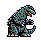
\includegraphics{./image/godzilla.png}
\end{center}
Ce qui nous donne sur la grille ceci : \\
\begin{center}
  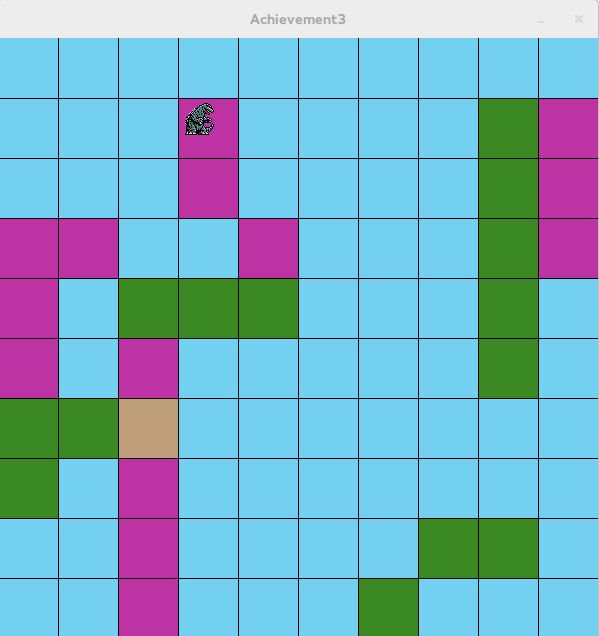
\includegraphics[scale=0.5]{./image/Godzilla_SDL.png}
\end{center}
\newpage
Dans l'affichage en console on va mettre une "*" après la valeur qui se trouve dans la grille comme dans l'exemple en position (9, 8) : \\
\begin{center}
  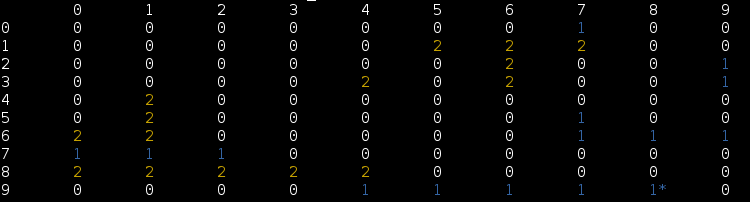
\includegraphics[scale=0.8]{./image/Godzilla_console.png}
\end{center}
\subsection{Fonctionnement de l'achievement3}
Dans notre grille, pour savoir si le monstre est présent, il se trouve à l'indice {\textit{NB\_JOUEURS}} + 1 dans notre tableau de case.\\
Pour réaliser cet achievement on a tout d'abord créer une structure Monstre qui possède :
\begin{itemize}
\item une Position afin de savoir où se trouve le monstre
\item un entier afin de savoir si le monstre a été agressé
\item un tableau d'entier de taille {\textit{NB\_JOUEURS}} pour savoir si le joueur i l'a agressé ou non
\end{itemize}
Puis ensuite il a fallu réaliser les fonctions pour les trois actions différentes qu'il peut réaliser.
\subsubsection{Monstre oblitère des cases}
Cette fonction consiste simplement à oblitérer les cases à gauche, droite, au dessus, en bas, sous le monstre si elles existent et s'il y a un bateau pour cela on utilise la fonction :
\begin{lstlisting}
int monstre_oblitere(struct Grille *grille, struct Monstre *monstre, struct Joueur *j1, struct Joueur *j2);
\end{lstlisting}
Cette fonction renvoie un entier qui correspond au nombre de case que le monstre a oblitéré. Cela nous permet de savoir si le monstre a oblitéré des cases ou si on doit faire l'autre action c'est à dire déplacer le monstre d'une case vers un bateau.\\
La complexité est en $\Theta(n)$ où n est le maximum entre le nombre de case en vie du joueur 1 et 2.
\subsubsection{Déplacement du monstre non agressé}
Cette fonction a pour prototype :
\begin{lstlisting}
void deplacement_monstre_pas_agresse(struct Joueur *j1, struct Joueur *j2, struct Monstre *monstre, struct Grille *grille);
\end{lstlisting}
Pour cette fonction, on a utilisé une fonction auxiliaire qui nous permet de savoir les cases les plus proches d'un monstre :
\begin{lstlisting}
void case_plus_proche_monstre(struct Joueur *j, struct Monstre *monstre, struct Position tab[], int *distance, int *nombre_case);
\end{lstlisting}
Cette fonction consiste à parcourir toutes les cases en vie du joueur et de regarder si la distance est inférieur à celle trouvée avant. Elle est de compléxité $\Theta(n)$ où est le nombre de case en vie du joueur.\\
On doit appliquer cette fonction pour les deux joueurs afin de trouver toutes les cases les plus proches.\\
Ensuite, on choisit une case aléatoire parmi toutes celles possibles et on se déplace d'une case vers elle.\\
La complexité de cette fonction est $\Theta(n + m)$ où n (resp. m) est le nombre de case en vie du joueur 1 (resp. 2). 
\subsubsection{Déplacement du monstre agressé}
Cette fonction a pour prototype :
\begin{lstlisting}
void deplacement_monstre_agresse(struct Grille *grille, struct Monstre *monstre, struct Joueur *j1, struct Joueur *j2, SDL_Surface *ecran, int affichage);
\end{lstlisting}
Premièrement, cette fonction teste si c'est le joueur 1 ou 2 ou les deux qui l'ont agressé afin de savoir vers quel joueur se déplacer. Pour savoir quel est le bateau le plus proche une fois le joueur choisi, on utilise la fonction : 
\begin{lstlisting}
int bateau_le_plus_proche(struct Monstre *monstre,  struct Joueur *j);
\end{lstlisting}
Cette fonction appelle la fonction {\textit{case\_plus\_proche\_monstre}} afin d'avoir la case la plus proche du monstre puis cherche à quel bateau elle appartient. \\
Puis une fois que la fonction {\textit{deplacement\_monstre\_agresse}} renvoie le bateau vers lequel le monstre doit se déplacer, elle fait appel à une fonction auxiliaire qui permet de lister toutes les cases autour des cases en vie du batal et en renvoie une aléatoirement parmi toutes elles. Cette fonction est :
\begin{lstlisting}
struct Position case_autour_du_batal(struct Batal *bat, struct Grille *grille);
\end{lstlisting}
La fonction pour déplacer un monstre agressé est en compléxité $\Theta(n)$ où est le nombre de case qu'occupe tous les batals.
\subsubsection{Tour du monstre}
\begin{lstlisting}
void monstre_qui_joue(struct Monstre *monstre, struct Grille *grille, struct Joueur *joueur1, struct Joueur *joueur2, SDL_Surface *ecran, int affichage){
  if(monstre->agresse)
    deplacement_monstre_agresse(grille, monstre, joueur1, joueur2, ecran, affichage);
  placer_monstre(monstre, grille);
  if(monstre_oblitere(grille, monstre, joueur1, joueur2))
    ;
  else
    deplacement_monstre_pas_agresse(joueur1, joueur2, monstre, grille);
  placer_monstre(monstre, grille);
}
\end{lstlisting}
Premièrement le monstre commence par regarder s'il a été attaqué ou non, si c'est le cas on utilise la fonction {\textit{deplacement\_monstre\_agresse}}. Ensuite, dans tous les cas, on utilise la fonction qui va oblitérer les cases, si elle oblitère des cases, on s'arrête là sinon on va alors appliquer la fonction qui permet de déplacer le monstre lorsqu'il n'est pas agressé.\\
\subsubsection{Affichage du chemin du monstre en SDL}
Pour afficher le chemin on part de la position de départ et on cherche d'abord à ce que le monstre arrive sur la même ligne que sa position d'arrivée. Par exemple si le monstre est en position (8, 2) et doit se rendre en (5, 4) il va se déplacer en (7, 2) puis (6, 2) puis (5, 2). Après on fait la même chose pour les colonnes. Si on reprend notre exemple il va donc aller en (5, 3) puis (5, 4). En SDL, l'affichage se fait comme ceci :
\begin{center}
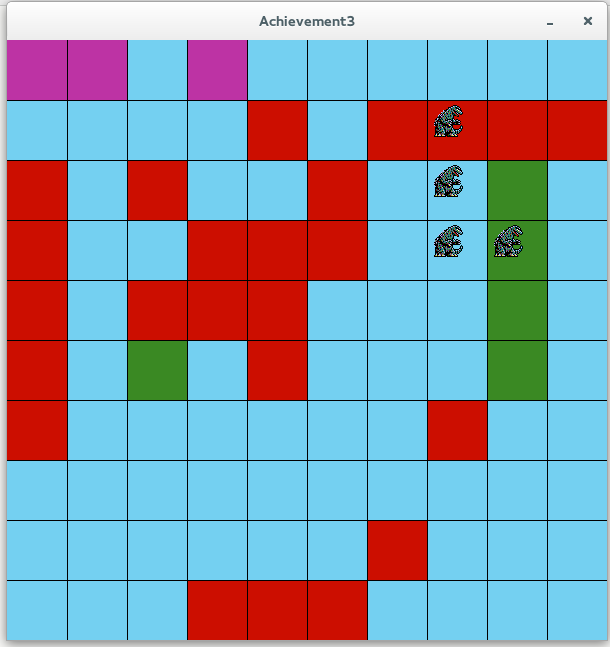
\includegraphics[scale=0.4]{./image/chemin_monstre_SDL}
\end{center}
\subsubsection{Fonctionnement de la boucle de jeu}
Notre fonction qui fait tourner la boucle de jeu a pour prototype :
\begin{lstlisting}
int achievement2(SDL_Surface *ecran, int affichage);
\end{lstlisting}
Elle prend un paramètre un écran si on utilise l'affichage SDL et un entier qui permet de savoir l'affichage souhaité et retourne un entier afin de nous dire le joueur qui a gagné.\\
Notre boucle de jeu tourne tant qu'il reste des bateaux des 2 joueurs et que le nombre de coup n'a pas dépassé la constante {\textit{NB\_COUP\_MAX}}. Dans notre boucle, on va :
\begin{itemize}
\item Déplacer un bateau du joueur1 si c'est possible.
\item Déplacer un bateau du joueur2 si c'est possible.
\item Calculer la position d'arrivée des torpilles pour les deux joueurs.
\item Oblitérer les cases si la position d'arrivée est possible(ie ne dépasse pas la distance maximale)
\item Effectuer le tour du monstre.
\item Incrémenter le nombre de coup
\end{itemize}
La fonction termine pour les mêmes raisons que dans l'achievement1 car notre structure de la boucle reste la même avec juste au début la possibilité de bouger les bateaux et le tour du monstre ce qui ne change pas la valeur de nb\_coup.
\subsection{Problèmes rencontrés}
\begin{itemize}
\item Le premier problème est lorsque le monstre est attaqué par le joueur 1 ou 2, ce n'est pas obligé qu'il puisse trouver un bateau de ce joueur vers lequel aller car il joue après la phase de tir. Comme dans l'exemple, s'il reste une case en vie pour chaque joueur, le joueur 1 attaque le monstre et le joueur2 détruit la dernière case en vie du joueur 1 alors lorsque le tour du monstre vient il ne peut pas se déplacer vers une case en vie du joueur 1 car il n'y en a plus. Donc ceci nous a contraint a modifier notre algorithme pour faire en sorte de ne pas avoir d'erreur si ce cas se produit.\\
\item Au début, on avait oublié d'enlever le monstre de la grille, donc on avait plusieurs monstres sur celle-ci.
\end{itemize}
